\chapter{Funzionamento dell'applicazione}
	\label{cap:funzionamento}		
In questo capitolo si illustreranno le modalità di funzionamento dell'applicazione implementata.
Come già detto nel capitolo~\ref{cap:progettazione}, l'applicazione si compone di due parti: server e client.

\section{Server}

Il server ha lo scopo di gestire gli utenti, i certificati relativi e di distribuire le chiavi di livello e le chiavi pubbliche degli utenti certificati.

L'applicativo può essere eseguito in due modi:
\begin{itemize}
	\item da riga di comando tramite l'istruzione:\\ \texttt{java -jar -DprogettoSII.configuration=<path-to-conf.properties> <path-to-jar>/server.jar};
	\item tramite l'IDE \emph{Eclipse} impostando opportunamente il percorso del file \texttt{conf.properties} nella configurazione di esecuzione (\textbf{Run Configuration}).  
\end{itemize}

Se l'applicazione viene lanciata da riga di comando è necessario inserire una password che serve a sbloccare il keystore. Dopo aver eseguito questo passaggio è possibile impartire comandi al server direttamente dal terminale. I comandi che sono disponibili ora sono: \texttt{quit} e \texttt{adminconf}.
Il primo chiude il server in maniera \emph{graceful} mentre il secondo avvia l'interfaccia grafica che consente all'amministratore di interagire con i dati degli utenti.
	\begin{center}	
		\begin{figure}[H]
		\centering
		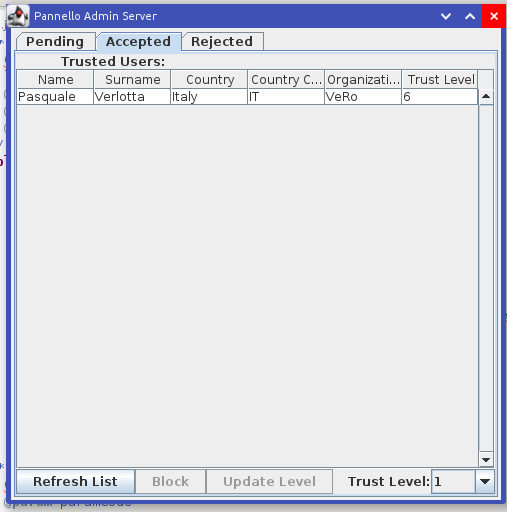
\includegraphics[scale=0.7]{Immagini/server_accepted}
		\caption[GUI del server]{Interfaccia grafica del server.}
		\label{fig:servergui}
		\end{figure}
	\end{center}
Come si vede nella figura~\ref{fig:servergui} ci sono tre schede riferite ad altrettante liste: 
\begin{itemize}
	\item \textbf{Pending} in cui compare la lista degli utenti che intendono registrarsi al sistema e attendono l'intervento dell'amministratore ;
	\item \textbf{Accepted} in cui c'è la lista degli utenti certificati che sono autorizzati all'accesso al sistema;
	\item \textbf{Rejected} in cui compare la lista degli utenti bloccati a cui è negato l'accesso.
\end{itemize}
I pulsanti in basso consentono di accettare o rifiutare o aggiornare le richieste degli utenti.

\section{Client}
Il client ha lo scopo di gestire le funzionalità di registrazione, login, cifratura e decriptazione.
La registrazione consiste nel riempire un form con dati anagrafici e i percorsi dei file delle cartelle necessarie per salvare i documenti cifrati/decifrati. Se la registrazione va a buon fine, cioè il server autentica l'utente, viene rilasciato un \textbf{SecureID}, che insieme con i dati inseriti viene scritto su un pdf generato automaticamente e salvato nella cartella di output scelta.
Il login consente di accedere all'applicazione e consiste nel riempire un form con Nome, Cognome, Password e il Codice rilasciato all'atto della registrazione. 

	\begin{center}	
		\begin{figure}[H]
		\centering
		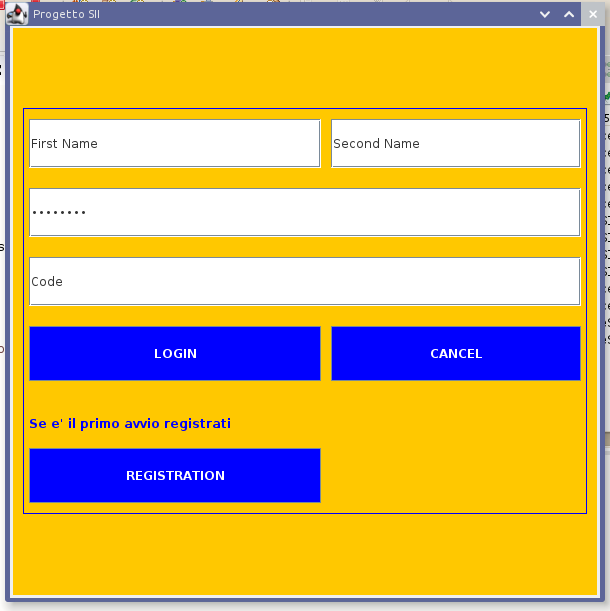
\includegraphics[scale=0.7]{Immagini/login}
		\caption[Login]{GUI di login}
		\label{fig:login}
		\end{figure}
	\end{center}
	
Dopo aver effettuato il login si accede alla schermata principale

	\begin{center}	
		\begin{figure}[H]
		\centering
		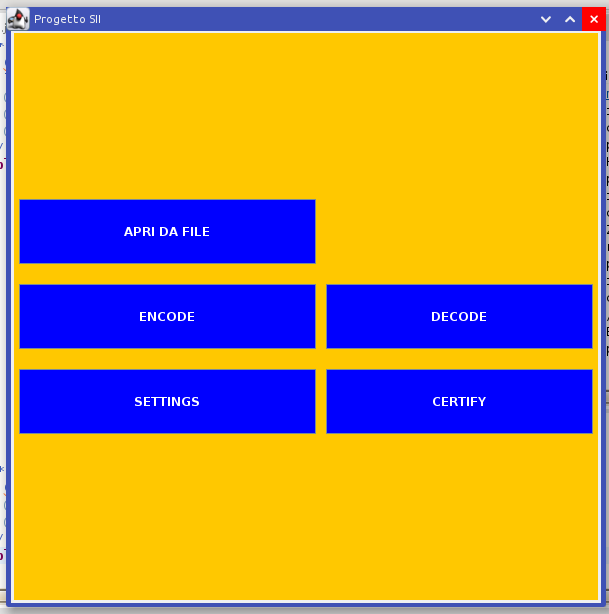
\includegraphics[scale=0.7]{Immagini/homelayout}
		\caption[homelayout]{GUI della schermata principale}
		\label{fig:home}
		\end{figure}
	\end{center}
	
Da questa schermata si accede alle funzionalità dell'applicazione cliccando i diversi pulsanti
\begin{itemize}
	\item \textbf{APRI} - consente di scegliere un file dal file system locale. Se il file scelto è un'immagine viene caricata la GUI per la decodifica, mentre se il file è un testo (.txt) viene caricata la GUI per la codifica;
	\item \textbf{ENCODE} - carica la GUI per la codifica;
	\item \textbf{DECODE} - carica la GUI per la decodifica;
	\item \textbf{CERTIFY} - la funzionalità necessaria per essere abilitati alla codifica e decodifica. Al primo login occorre, infatti, scaricare il certificato dal server, se l'amministratore ha autorizzato l'utente, ed aggiornarne i dati. 
\end{itemize}

\subsection{Cifratura}
La seguente figura~\ref{fig:encode} illustra la GUI per la composizione di un file da criptare. Vi si accede cliccando \textbf{ENCODE} nella schermata principale, e selezionando un file.

	\begin{center}	
		\begin{figure}[H]
		\centering
		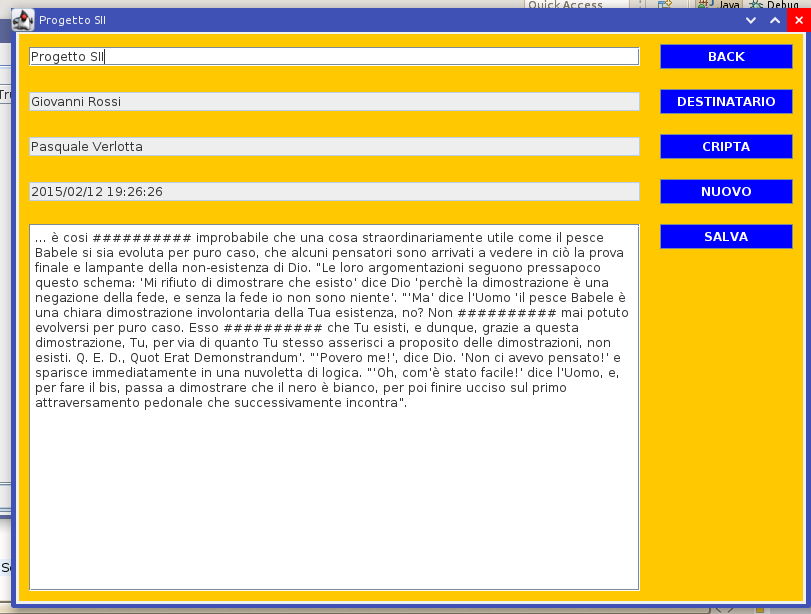
\includegraphics[scale=0.6]{Immagini/writelayout}
		\caption[GUI di encode]{Intefaccia grafica per la codifica}
		\label{fig:encode}
		\end{figure}
	\end{center}
	
La schermata si compone di cinque campi:
\begin{itemize}
	\item Il \textbf{titolo}  che comparirà nell'intestazione del documento;
	\item L'\textbf{autore} del documento, che viene riempito in automatico con il nome e cognome dell'utente loggato;
	\item Il \textbf{destinatario} che viene impostato tramite il pulsante \textbf{DESTINATARIO}, che consente di scegliere se cifrare per un singolo utente, o per un livello;
	\item Le \textbf{informazioni} che per il momento consistono in data e ora della creazione del documento;
	\item L'area nella quale verrà inserito automaticamente il testo preso dal file selezionato.
\end{itemize}
e di cinque pulsanti, con funzioni autoesplicative. 

Una volta selezionato il destinatario del documento si seleziona il testo da cifrare e si preme il pulsante \textbf{CRIPTA} che esegue la cifratura tramite RSA con la chiave pubblica del destinatario o tramite AES con le chiavi di livello, partendo dal livello 1 fino al livello scelto, ed infine sostituisce il testo selezionato con una serie di hashtag.
Il pulsante \textbf{SALVA} genera il QR-Code contente la firma del documento cifrata, il QR-Code con le informazioni in chiaro per decriptare, e i QR-Code relativi alle parti di testo criptate. Una volta terminata la cifratura viene generata l'immagine come descritto nel capitolo \ref{cap:progettazione}.

\subsection{Decifrazione}
La seguente figura~\ref{fig:decode} illustra la GUI per la composizione di un file da decriptare. Vi si accede cliccando \textbf{DECODE} nella schermata principale, e selezionando un file.
	
	\begin{center}	
		\begin{figure}[H]
		\centering
		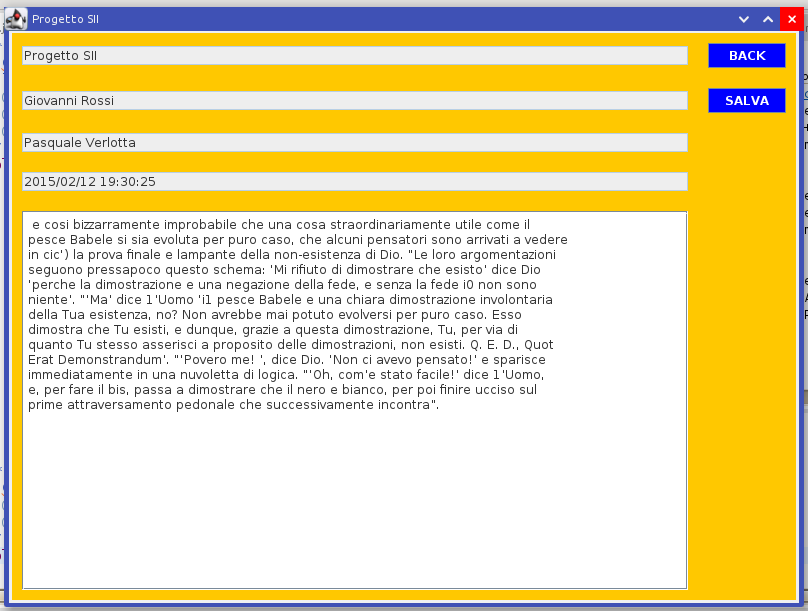
\includegraphics[scale=0.6]{Immagini/readlayout}
		\caption[GUI di decode]{Interfaccia grafica per la decodifica}
		\label{fig:decode}
		\end{figure}
	\end{center}

La GUI ha gli stessi campi della GUI per l'encode, con la differenza che questi sono riempiti in automatico dal sistema in fase di decriptazione del documento e il testo è in chiaro, decriptato quindi.
Nel caso il testo contenga ancora gli hashtag significa che non si ha il privilegio di decriptare il file, perché o non si ha il livello autoritativo necessario o non si è il destinatario del documento.